%!TEX encoding = UTF-8 Unicode
%!TEX root = ../galgas-book.tex

%--------------------------------------------------------------
\chapterLabel{Projet \texttt{Xcode} et application Cocoa}{appliCocoa}
%-------------------------------------------------------------

Vous pouvez demander à GALGAS d'engendrer un projet \texttt{Xcode}, qui contiendra :
\begin{itemize}
  \item le compilateur en version \emph{release} sous la forme d'un utilitaire en ligne de commande ; 
  \item le compilateur en version \emph{debug} sous la forme d'un utilitaire en ligne de commande ; 
  \item une application Cocoa permettant d'appeler les deux utilitaires.
\end{itemize}






\section{Paramétrage du projet GALGAS}

Pour engendrer un projet \texttt{Xcode}, il vous suffit d'ajouter une déclaration telle que \ggs+%Mavericks+ dans votre fichier projet (d'extension \tpp{.galgasProject}, voir \refChapterPage{composantProjet}). Par exemple :

\begin{galgas}
project (0:0:1) -> "logo" {
  %Mavericks
  %applicationBundleBase : "fr.what"
  ...
\end{galgas}

Un projet \texttt{Xcode} définit la version de Mac OS pour laquelle il va être compilé : ainsi, \ggs+%Mavericks+ définit la version \texttt{Mavericks} (10.9). Le \refTableau{options-pour-xcode} liste les différents options possibles. GALGAS fixe la version indiquée dans le projet \texttt{Xcode}, et il faut ensuite que la version de \texttt{Xcode} utilisée soit compatible avec ce réglage. L'option \ggs+%LatestMacOS+ correspond au réglage correspondant du projet \texttt{Xcode} engendré. Quand \ggs+%SnowLeopard+ est sélectionné, l'application Cocoa engendrée utilise le \emph{garbage collector}. Sinon, elle adopte l'\emph{Automatic Reference Counting} (\emph{ARC}).

Il y a une seconde option à ajouter dans le projet GALGAS : \ggs+%applicationBundleBase+. Celle-ci fixe le \emph{Bundle Identifier} de l'application Cocoa. À la chaîne définie dans l'option (ici \ggs+"fr.what"+) est ajouté le nom du projet (défini dans l'en-tête, ici \ggs+"logo"+), précédé par un point : le \emph{Bundle Identifier} est donc \tpp{fr.what.logo}.


\begin{table}[t]
  \centering
  \begin{tabular}{rlll}
    \textbf{Option} & \textbf{Version SDK Mac OS} & \textbf{Version de}  &  \textbf{Gestion mémoire}\\
                    &                             & \textbf{déploiement} &                          \\
    \ggs+%SnowLeopard+ & \texttt{SnowLeopard} (10.6) & 10.6  & \emph{Garbage Collector}\\
    \ggs+%Lion+ & \texttt{Lion} (10.7) & 10.7 & \emph{ARC}\\
    \ggs+%MountainLion+ & \texttt{Mountain Lion} (10.8) & 10.8 & \emph{ARC}\\
    \ggs+%Mavericks+ & \texttt{Mavericks} (10.9) & 10.9 & \emph{ARC}\\
    \ggs+%Yosemite+ & \texttt{Yosemite} (10.10) & 10.10  & \emph{ARC}\\
    \ggs+%YosemiteElCapitan+ & \texttt{El Capitan} (10.11) & 10.10  & \emph{ARC}\\
    \ggs+%ElCapitan+ & \texttt{El Capitan} (10.11) & 10.11  & \emph{ARC}\\
    \ggs+%Sierra+ & \texttt{Sierra} (10.12) & 10.12  & \emph{ARC}\\
    \ggs+%LatestMacOS+ & -- & -- & --\\
  \end{tabular}
  \caption{Options du projet GALGAS indiquant la version Mac OS}
  \labelTableau{options-pour-xcode}
  \ligne
\end{table}







\section{Projet \texttt{Xcode} engendré}


Quand le projet GALGAS est compilé, un répertoire \tpp{xcode-project} directory est créé, et contient :
\begin{itemize}
\item le fichier projet \texttt{Xcode} ;
\item un fichier \tpp{build.command} ;
\item un fichier \tpp{Info.plist} ;
\item un répertoire \tpp{English.lproj} ;
\item un répertoire \tpp{userResources}.
\end{itemize}

Le rôle de chacun est précisé par le \refTableau{fichiers-repertoires-xcode}. Ne pas modifier ces fichiers et répertoires à la main, une compilation GALGAS supprimerait vos changements. La seule exception est le contenu du répertoire \tpp{userResources} qui n'est pas modifié par les compilations GALGAS.

\begin{table}[t]
  \centering
  \begin{tabular}{rp{11cm}}
    \textbf{Fichier ou répertoire} & \textbf{Rôle}\\
    \tpp{build.command} & Effectue la compilation Xcode, appelable via une commande \emph{Shell} \\
    \tpp{Info.plist}    & Informations pour l'application Cocoa \\
    \tpp{English.lproj} & Informations pour l'application Cocoa \\
    \tpp{userResources} & Permet d'associer des icônes aux fichiers sources de votre compilateur, ainsi qu'à l'application Cocoa engendrée (voir \refSectionPage{ajouterIconesAppliCocoa}) \\
  \end{tabular}
  \caption{Fichiers et répertoires relatifs au projet Xcode}
  \labelTableau{fichiers-repertoires-xcode}
  \ligne
\end{table}





\sectionLabel{Définir des icônes pour votre application Cocoa}{ajouterIconesAppliCocoa}

Vous pouvez définir :
\begin{itemize}
  \item une icône pour l'application Cocoa ;
  \item une icône particulière pour chaque type de fichier source.
\end{itemize}

Le nom de chaque fichier d'icône fixe son rôle :
\begin{itemize}
  \item pour l'application Cocoa, le fichier d'icône doit s'appeler \tpp{application\_icns.icns} ;
  \item pour chaque type de fichier source, le nom est basé sur l'extension du fichier : si celui-ci est par exemple \tpp{.logo}, le fichier d'icônes doit s'appeler \tpp{logo\_icns.icns}.
\end{itemize}

Ces fichiers d'icônes doivent être placés dans le répertoire \tpp{userResources}, et il faut ensuite refaire une compilation GALGAS pour que ces fichiers soient ajoutés au projet \texttt{Xcode}.

En résumé :
\begin{enumerate}
  \item concevoir les fichiers d'icônes, en fixant leur nom comme indiqué ci-dessus ;
  \item placer ces icônes dans le répertoire \tpp{userResources} ;
  \item effectuer une compilation GALGAS : celle-ci met à jour le projet \texttt{Xcode}, en ajoutant les fichiers d'icônes au \emph{target} Cocoa ;
  \item recompiler le \emph{target} Cocoa du projet \texttt{Xcode} : les icônes sont prises en compte.
\end{enumerate}











%\sectionLabel{Customizing Syntax Coloring}{customizingSyntaxColoring}
%
%This feature enables to set particular display attributes to a given list of tokens. This list is defined by a plist file located in the \emph{Resources} directory of the application bundle.
%
%{1} Edit the GALGAS lexique component, and add one (or more) \ggs+style+ entries. For example:
%
%\begin{galgas}
%lexique my_lexique :
%  ...
%style mySpecificStyle -> "My Style" ;
%  ...
%end lexique ;
%\end{galgas}
%
%This new style's feature can be edited as other styles, by the Preferences setting of your Cocoa application.
%
%
%{2} Create a plist file with the \emph{Property List Editor} application. This file should be named with the lexique component name, suffixed by \tpp{-syntax-coloring-adds}: so, for the example, the file name is \tpp{my\_lexique-syntax-coloring-adds.plist}. Put this file in the \emph{userResources} directory: so when the GALGAS project document is compiled, this file is added to the Cocoa Target of the Xcode project. 
%
%{3} Edit the \tpp{my\_lexique-syntax-coloring-adds.plist} with the \emph{Property List Editor} application or Xcode. Add one entry for every custom syntax coloring case: the \emph{key} is the terminal spelling, the \emph{value} has the \emph{String} type, and the specific style name. For example, the \refFigure{}{customSyntaxColoringPropertyList} shows the assignment of the terminal which spelling is \tpp{begin} by the \tpp{mySpecificStyle} style.
%
%\begin{figure}[t]
%  \centering
%  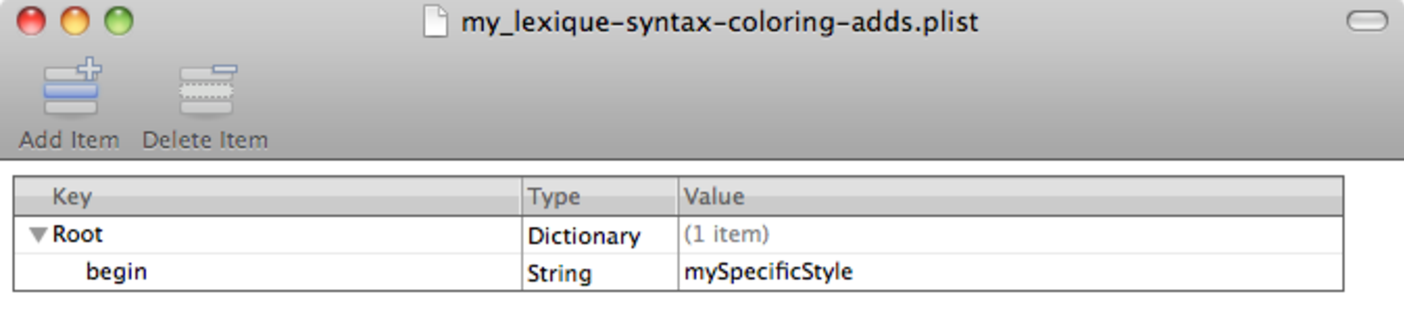
\includegraphics[width=15cm]{chapter-cocoa-features/custom-syntax-coloring-property-list-edition.pdf}
%  \caption{Example of a syntax coloring property list}
%  \labelFigure{customSyntaxColoringPropertyList}
%  \ligne
%\end{figure}
%
%If your provides an undefined style name, you will be warned every time you open a document by a beep and a small explanation window.






\sectionLabel{Indexation des fichiers sources}{indexingYourSourceFiles}

Vous pouvez configurer votre projet GALGAS pour que l'application Cocoa engendrée établisse une indexation et des références croisées : un \tpp{cmd-click} affiche un menu contextuel. Cette indexation est basée sur l'analyse syntaxique. C'est ce qui a été fait pour l'application \texttt{CocoaGalgas} (\refFigure{}{indexingUnderCocoaGALGAS}). On voit dans le menu contextuel trois classes d'index : \tpp{Class Definition}, \tpp{Class Reference as Superclass} et \tpp{Abstract Category Method Definition} ; au dessous, les références croisées correspondantes.


%You can configure your project for enabling cross-referencing entities with your Cocoa application. This has been done in GALGAS, providing such feature (\refFigure{}{indexingUnderCocoaGALGAS}). The contextual menu is displayed with a \texttt{cmd-click}.

\begin{figure}[t]
  \centering
  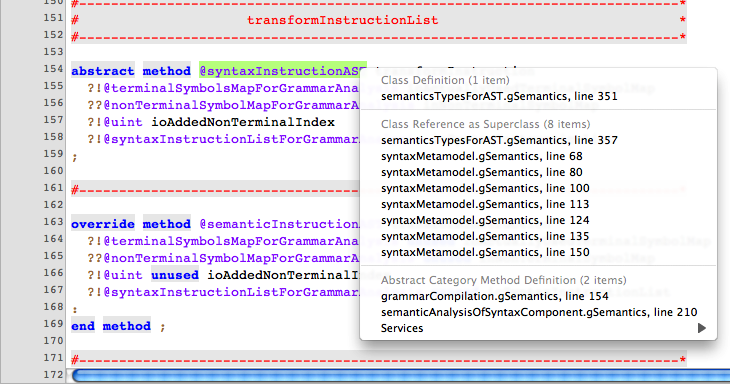
\includegraphics[width=16cm]{chapter-cocoa-features/indexing-sample.png}
  \caption{Indexation et références croisées dans l'application CocoaGalgas}
  \labelFigure{indexingUnderCocoaGALGAS}
  \ligne
\end{figure}

Pour configurer votre projet, vous avez à modifier le composant \emph{lexique}, le composant \emph{syntax}, le composant \emph{grammar}, et la règle d'analyse du fichier source. Les cinq modifications sont présentées successivement ci-après, en prenant comme exemple le langage LOGO (\refSectionPage{presentation-logo}).





\subsection{En tête du composant \texttt{lexique}}

Il faut modifier l'en-tête, en ajoutant la déclaration  \ggs+indexing in+ :


\begin{galgas}
lexique logo_lexique indexing in "INDEXING" {
  ...
\end{galgas}

La chaîne \ggs+"INDEXING"+ définit le nom du répertoire qui contient les fichiers cache de l'indexation. Ce répertoire est relatif au répertoire qui contient le fichier source.

Note : si vous effectuez maintenant la compilation GALGAS, vous obtiendrez une erreur sur la définition de la grammaire, indiquant qu'elle doit aussi indiquer la prise en compte de l'indexation.




\subsection{En tête du composant \texttt{grammar}}

Il suffit de préfixer par \ggs+indexing+ l'en-tête du composant \ggs+grammar+ :

\begin{galgas}
indexing grammar logo_grammar ... {
  ...
\end{galgas}

Note : maintenant, la compilation GALGAS s'effectue sans erreur.




\subsection{Règle d'analyse des fichiers sources}

La règle d'analyse des fichiers source doit mentionner dans l'en-tête la grammaire utilisée pour l'analyse (pour l'exemple du langage LOGO, c'est le rôle de la troisième ligne \ggs+grammar logo_grammar+).

\begin{galgas}
case . "logo"
message "a source text file with the .logo extension"
grammar logo_grammar
?sourceFilePath:@lstring inSourceFile {
  grammar logo_grammar in inSourceFile
}
\end{galgas}

Quand le mode d'exécution (absence de l'option \tpp{-{}-mode}) est le mode par défaut, les instructions de la règle sont exécutées. Ci-dessus, la seule instruction est l'instruction \ggs+grammar logo_grammar in inSourceFile+ (ligne 5).

Quand le mode d'exécution (présence de l'option \tpp{-{}-mode}) n'est pas le mode par défaut, les instructions de la règle ne sont pas exécutées, et les opérations sont guidées par la grammaire indiquée ligne 3. Dans le cas de l'indexation, l'exécution construit l'indexation du fichier source.









\subsection{Déclaration des classes d'index}

La déclaration des classes d'index s'effectue dans l'analyseur lexical. Dans la cadre du langage d'exemple LOGO, on veut simplement indéxer les routines, plus précisément l'endroit de leur définition, et les endroits où elles sont appelées. On définit donc deux classes d'index \ggs+routineDefinition+ et \ggs+routineCall+. À chaque déclaration est associée une chaîne de caractères, qui sera le titre affiché dans le menu contextuel. 


\begin{galgas}
lexique logo_lexique indexing in "INDEXING" {
  ...
indexing routineDefinition : "Routine Definition"
  ...
indexing routineCall : "Routine call"
  ...
\end{galgas}


Ces définitions peuvent être placées à tout endroit dans la définition de l'analyseur lexical.








\subsection{Définition des entrées indexées}

L'analyseur syntaxique va être complété de façon à définir les symboles qui seront indéxés. Plus précisement, c'est l'instruction d'analyse de symbole terminal qui est modifiée.

Considérons d'abord la déclaration de routine. La règle de l'analyseur syntaxique qui définit cette analyse est :

\begin{galgas}
rule <routine_definition> {
  $ROUTINE$
  $identifier$ ?let routineName
  $BEGIN$
  <instruction_list>
  $END$
}
\end{galgas}

Le nom de la routine est défini par l'instruction \ggs+$identifier$ ?let routineName+ : on la modifie alors de façon à signifier que l'indentificateur doit être indéxé comme une définition de routine :

\begin{galgas}
rule <routine_definition> {
  $ROUTINE$
  $identifier$ ?let routineName indexing routineDefinition
  $BEGIN$
  <instruction_list>
  $END$
}
\end{galgas}

Maintenant, l'instruction d'appel de routine :

\begin{galgas}
rule <instruction> {
  select
    $CALL$
    $identifier$ ?let @lstring routineName
    $;$
  or
    ...
  end
}
\end{galgas}

On modifie de manière analogue l'instruction \ggs+$identifier$ ?let @lstring routineName+ :

\begin{galgas}
rule <instruction> {
  select
    $CALL$
    $identifier$ ?let @lstring routineName indexing routineCall
    $;$
  or
    ...
  end
}
\end{galgas}



\subsection{Compilation et essai}

Les modifications sont terminées. Vous pouvez recompiler votre projet (compilation GALGAS puis compilation de la cible Cocoa du projet \texttt{Xcode}). La \refFigure{}{exemple-indexation-logo} montre le résultat obtenu en effectuant un \tpp{cmd-click} sur le nom de la routine.

\begin{figure}[t]
  \centering
  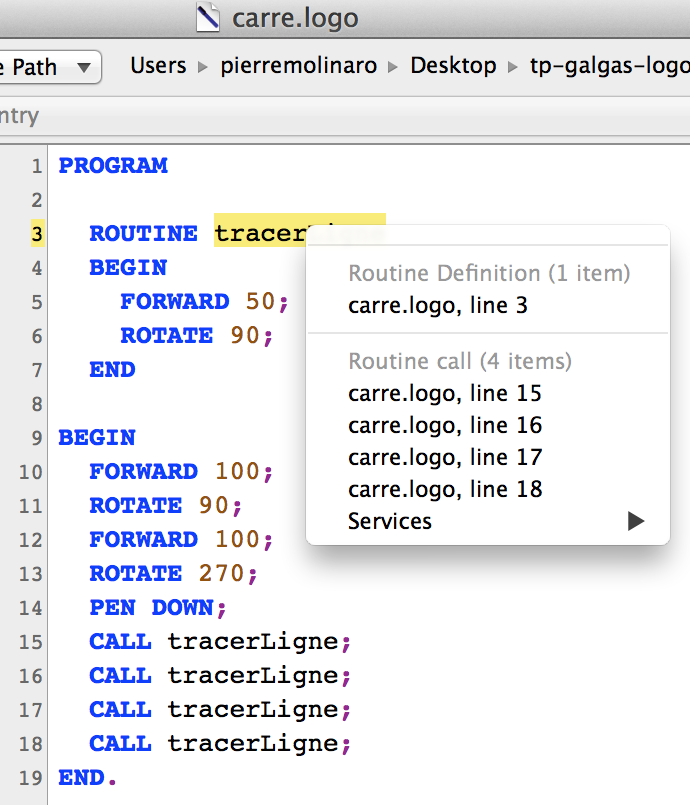
\includegraphics[width=8cm]{chapter-cocoa-features/exemple-indexation-logo.png}
  \caption{Exemple d'indexation en LOGO}
  \labelFigure{exemple-indexation-logo}
  \ligne
\end{figure}



%\noindent{4} \textbf{Program component configuration.} Insert the \ggs+grammar+ declaration after the « \texttt{message ...} » declaration in every program rule concerned by indexing:
%
%\begin{galgas}
%case ...
%message ...
%grammar my_grammar
%?@lstring inSourceFile {
%  ...
%\end{galgas}
%
%
%
%
%
%
%\noindent{5} \textbf{Define indexing entries.} The indexing entries are defined within the rules of syntax components. The \emph{terminal check} instruction is the unique way for definition, by naming an index class name:
%
%\begin{galgas}
%syntax ... ("my_lexique.gLexique") :
%  ...
%rule ... :
%  ...
%  $identifier$ ? ... indexing myIndexClass1 ;
%  ...
%end rule ;
%  ...
%\end{galgas}
%
%Any kind of terminal symbol accepts an « \texttt{indexing} » attribute : keywords, delimiters, literal string, integers, identifiers, \dots
%
%Several index class names can be named, using a comma as separator:
%\begin{galgas}
%  ...
%  $identifier$ ? ... indexing myIndexClass1, myIndexClass2 ;
%  ...
%\end{galgas}
%
%
%
%
%
%
%\noindent{6} \textbf{Compile and play.} Now, you can compile and run the Cocoa Application. With a \texttt{cmd}-click on an indexed terminal symbol, the contextual menu is displayed. You can delete the indexing directory at any moment, it will be rebuilt as needed.







